\documentclass{article} % For LaTeX2e
\usepackage{nips15submit_e,times}
\usepackage{hyperref}
\usepackage{graphicx}
\usepackage{amsmath}
\usepackage{amsthm}
\usepackage{graphicx}
\usepackage{caption}
\usepackage{subcaption}
\usepackage{lmodern}
\usepackage{titlesec}
\usepackage{longtable}
\usepackage{geometry}
\usepackage{multirow}
\usepackage{listings}
\usepackage{amsfonts}
\usepackage{algorithm}
\usepackage{algpseudocode}
\usepackage{multirow}
\usepackage{array}
\usepackage{url}

\author{
Thomas Nedelec \\
MSc Machine Learning\\
\texttt{thomas.nedelec.15@ucl.ac.uk} \\
\And
Michal Daniluk \\
MSc Machine Learning\\
\texttt{michal.daniluk.15@ucl.ac.uk} \\
}
\title{Supervized Learning: Assignment 1}




\newcommand{\fix}{\marginpar{FIX}}
\newcommand{\new}{\marginpar{NEW}}

\nipsfinalcopy % Uncomment for camera-ready version

\begin{document}


\maketitle

\section{Exercise 1: Least Square Regression: effect of the training set size}
We generated a noisy random data set, containing 600 samples, as $y_i = x_i'w + n_i$, where each $x_i$ and $n_i$ are drawn from the standard normal distribution. We splitted the data into a training set of size 100 a test set of size 500. We compute the mean squared error on both the training and test sets. Figure \ref{fig:lsr} shows examples of different training sets and estimated regression $w$.

 \begin{figure}[H]
\center
\begin{tabular}{ccc}
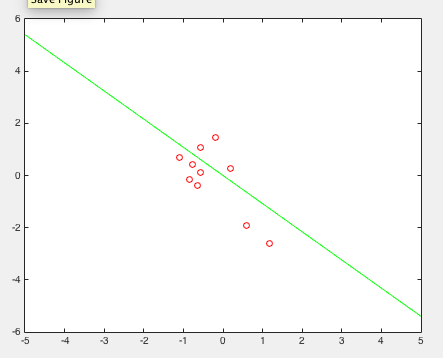
\includegraphics[width=0.3\textwidth]{10points}&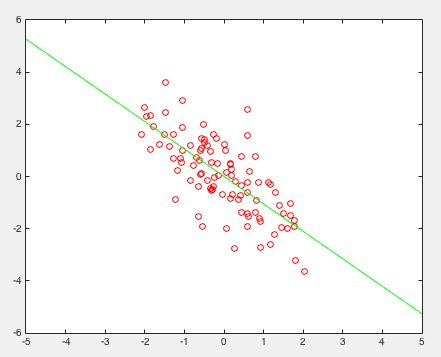
\includegraphics[width=0.3\textwidth]{100points}&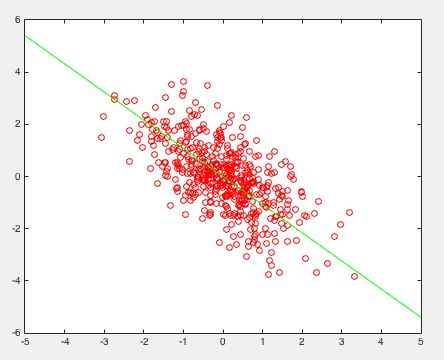
\includegraphics[width=0.3\textwidth]{500points}
\end{tabular}
\caption{ (a) training set of 10 points (b) training set of 100 points (c) the entire data set}
\label {fig:lsr}
\end{figure} 

Figure \ref{fig:resultMatrix1} illustrates the ''2 x 2'' table of averages mean square error for both training and test sets, on both 10 and 100 element-size training set.
\begin{figure}[H]
\begin{center}
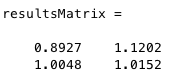
\includegraphics[width=0.4\textwidth]{resultsMatrix}
\end{center}
\caption{Average mean square error for both training and test sets, on both 10 and 100 element-size training set.}
\label{fig:resultMatrix1}
\end{figure}

We can observe that increasing the size of training set lets to decrease the average mean error on the test set.
However, it increased the average mean error on train set.
With increasing the size of training set, the average error on the test and train set became similar.
The average error on test set is larger than on train set. It is clear, beacause we have seen the train data before and haven't seen the test data.
\section{Exercise 2: Least Square Regression: effect of dimensionality}
We repeated the task in exercise 1, but with 10-dimensional data sets. Figure \ref{fig:resultMatrix2} illustrates the ''2 x 2'' table of averages mean square error for both training and test sets, on both 10 and 100 element-size training set.
\begin{figure}[H]
\begin{center}
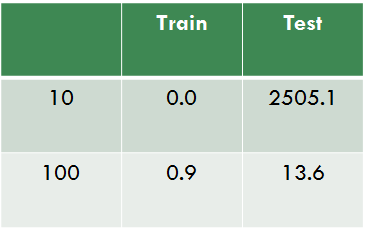
\includegraphics[width=0.4\textwidth]{resultsMatrix2}
\end{center}
\caption{Average mean square error for 10-dimensional data for both training and test sets, on both 10 and 100 element-size training set.}
\label{fig:resultMatrix2}
\end{figure}

For 10-sample training set, we obain the average mean square error $0$ for train set and $2505.1$ for test set. We have 10-dimensional data and 10 samples, so we can accurately predict $y_i$ without any errors. However, the prediction is overfitted to the training data and we have a large error for test set. Icreasing number of samples to 100 helps to decrease average error on test set. Average error for train set is bigger than for 10 samples, but our goal is to decrase test error.

\section{Ridge regression}

The regularization is a way to reduce the freedom of the classifier in order to improve the generalization and reach a better test set average error. 
\\ To implement ridge regression, we would like to minimize according to \textit{w} the cost function, 
\begin{equation}
\gamma w^{T}w + \frac{1}{l} \sum_{i=1}^{l}(x_{i}^{T}w - y_{i})^{2}.
\end{equation}
Using the notation $X=(x_{1}, x_{2},...,x_{l})^{T}$, a matrix containing the training sample vectors as its rows, we can rewrite the cost function as: 
\begin{equation}
\gamma w^{T} w + \frac{1}{l} Tr((Xw - Y)^{T}(Xw - Y))
\end{equation}
Taking derivative according to w, we reach: 
\begin{equation}
2\gamma w + 2 \frac{1}{l} (X^{T}Xw - 2Y^{T}X)=0
\end{equation}
To reach the conditions for optimality, we set the previous equation to zero and we reach: 
\begin{equation}
w=(\gamma l Id +X^{T}X)^{-1}Y^{T}X
\end{equation}
because if $\gamma*l \ne 0$ $(\gamma l Id +X^{T}X)$ is non-singular.

$\gamma l Id +X^{T}X $ is symetric.

We consider $u \in \mathbb{R}^{d}$:
\begin{align*}
\langle (\gamma l Id +X^{T}X)u,u \rangle &= \langle \gamma l u,u \rangle + \langle X^{T}X,u \rangle
\\  &= \gamma l \langle  u,u \rangle + \langle X u, X u \rangle
\\ &= \gamma l ||u||^{2} + ||Xu||^{2} > 0 \textit{ for u $\ne$ 0}
\end{align*}
Thus $\gamma l Id +X^{T}X$ is definite positve. 

\section{Effect of the regularisation parameter}

  \begin{figure}[H]
\center
\begin{tabular}{cc}
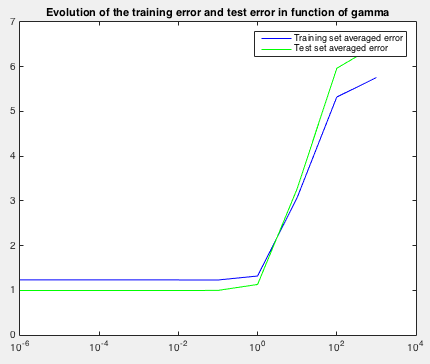
\includegraphics[width=0.5\textwidth]{error4}&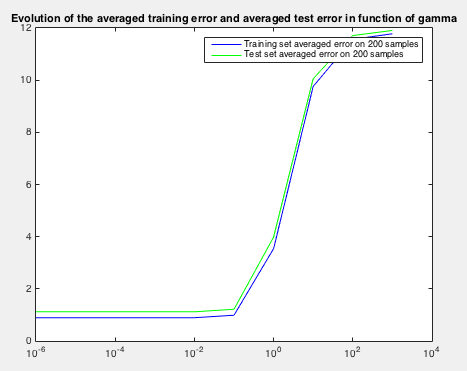
\includegraphics[width=0.5\textwidth]{averagederror4}
\end{tabular}
\caption{ (a) evolution of the training error and test errror for one run (b) evolution of the training error and test error averaged on 200 runs}
\end{figure}

First, the graph shows that if gamma is too high, the training error and test error increase dramatically. It is intuitive because when gamma is high the algorithm is far more likely to minimize $||w||$  rather than the training error.


We have an optimal point corresponding to inflection point of the curve in order to select $\gamma$. Nevertheless, the training set error is not a sufficiently good guidance to select the regularization parameter because the charts are quite different. 

However, when we average the training error on 200 runs, we can observe that now the test error and the training error are now almost identical.

A way to select the optimal $\gamma$ would be to plot the error on the training set averaged on a certain number of runs of the algorithm and select the optimal $\gamma$ on this curve. 


\section{Tuning the regularization parameter using a validation set}

\section{Tuning the regularization parameter using cross valdidation}
We use 5-fold cross validation to tune the regularization parameter. Figure \ref{fig:ex6} shows cross-validation score on top of the training and test set error for different values $\gamma = \{10^{-6}, 10^{-5}, \dots, 10^3 \}$ of the regularization parameter.

\begin{figure}
    \centering
    \begin{subfigure}[b]{0.45\textwidth}
        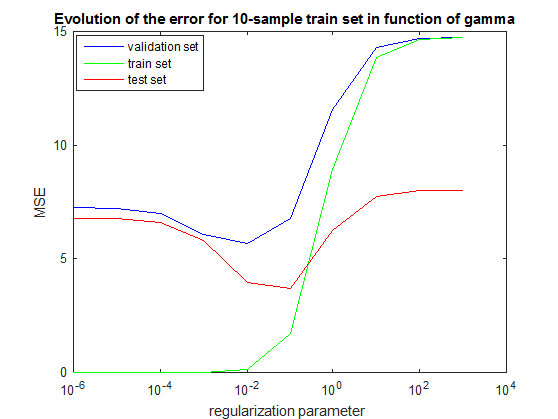
\includegraphics[width=\textwidth]{ex6_10}
        \caption{10-sample training set}
    \end{subfigure}
    \begin{subfigure}[b]{0.45\textwidth}
        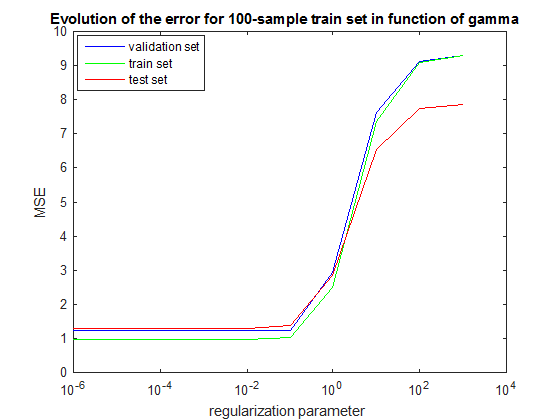
\includegraphics[width=\textwidth]{ex6_100}
        \caption{100-sample training set}
    \end{subfigure}
    \caption{Evaluation of the mean square error in function of gamma for different number of training examples.}
    \label{fig:ex6}
\end{figure}
 TO DO :
Interpretation
\end{document}
